\chapter{Online Learning}
\label{ch:bg-online-learning}

In this chapter we will provide an introduction to online learning, which is the learning
setting for Papers \uncertaintreesNum and \boostvhtNum. We start by providing a brief
overview of the kinds of models available for online learning in Section \ref{sec:bg-ol-models}.
Since our work focuses on decision trees and ensemble methods we present an overview of
the state of the art in Sections \ref{sec:bg-dt-online-trees} and \ref{sec:bg-ol-ensembles} respectively.
We identify issues and solutions for the evaluation of online models in Section \ref{sec:bg-ol-evaluation}, and conclude the chapter with a look at the available
open-source software for online learning in Section \ref{sec:bg-ol-software}.

\section{Models}
\label{sec:bg-ol-models}

As with batch learning, a wide range of models exists in the online
learning domain. Commonly, these are models that were first developed
for the batch setting and subsequently adapted to online learning.
In this section we focus on supervised learning methods for
classification and regression, and explore different
learning representations to demonstrate the variety of
models available for online learning, following the
classification in \cite{onlineML}. For a comprehensive
introduction to the various models available in streaming
learning we refer the reader to \cite{moa-book}.
An important aspect of online learning that we do not cover in this chapter is learning
under concept drift, that is, when the underlying distribution
of the data changes during learning. We refer the reader
to the surveys \cite{concept-drift-survey-indre, concept-drift-survey-gama}
for in-depth looks at the topic.

\subsection*{Instance Based Learning}
One of the simplest and most intuitive methods in machine learning
is Instance Based Learning (IBL), which usually takes the form of
a nearest neighbor model.
In Instance Based Learning, we make predictions based on the instances themselves, unlike
model-based approaches that try to extract a model (function) from the
data. IBL exemplifies many characteristics
that make it a good candidate for online learning, and the
IBLStreams work of \citet{ibl-streams} demonstrates how these
can be put to use to create an efficient online learning model.
IBL algorithms are inherently incremental, and can be faster to
update compared to a model-based approach, but they suffer from two
distinct disadvantages: First, they need to store the data points themselves, which in a
massive streaming data scenario can be infeasible. To deal with this
issue IBLStreams will evict the oldest examples once an upper limit on
the number of data points stored is reached. Second, inference can be much slower as it requires
finding the k nearest neighbors to the incoming dataset, which even when
using efficient indexing structures (like Locality Sensitive Hashing~\cite{lsh-indyk, lsh-gionis}) can be very costly
compared to a model-based prediction, e.g. from a linear model.
\citeauthor{ibl-streams} suggest that IBL makes more sense in scenarios where updates are
often but queries infrequent.

In terms of drift adaptation, IBLs can have
the advantage that removing the effect of older data points is easy
compared to say an ANN model, but it is still highly model-dependent.
The authors suggest different ways to deal with
concept drift in IBLStreams. They mention the limitations of a non-adaptive, window-based
approach and suggest that IBL methods are good candidates for learning
under drift because of their locality property, that is, that introducing
a new example will only affect the predictions made around that region.
In theory, an example should only be included in the model if it improves the
accuracy, but that is impossible to know ahead of time. However, one can use heuristics
to determine when to discard examples. These include the temporal and/or spatial
relevance, or consistency of the examples to the current concept.
In IBLStreams, the contents and size of the ``case base'',
i.e. the examples that form the nearest neighbor representation, is
updated automatically. IBLStreams tries to maintain a balance between
maintaining few examples in the case base in order to be able to deal
easier with concept drift, while keeping the set large enough so that
predictions under a single concept are accurate. To that end, they
use statistical change detection mechanisms and also provide ways
to update the parameters of the algorithm, e.g. the number of nearest
neighbors to examine, based on the observed error.

\subsection*{Linear Models}
In terms of model-based approaches, linear models are popular
for online learning due to their simplicity, efficiency and interpretability.
For regression these models have the general form~\cite{esl}:

\begin{equation}
	f(X) = \beta_0 + \sum_{j=1}^{p}{X_j\beta_j}
\end{equation}

\noindent
where $p$ is the number of features in the dataset, where a linear relationship is assumed between the dependent and independent predictors.

One of the earliest examples of an online linear classification model is the seminal
Perceptron algorithm \cite{perceptron} that tries to find a separating hyperplane
between two classes based on the distance of the misclassified points to the
decision boundary~\cite{esl}.
In the online setting, linear models are typically trained using a form
of stochastic gradient descent, that moves the coefficients
of the model according to the gradient of a single data point
and a step size parameter.
The Perceptron is a simple algorithm that however has many drawbacks
noted by \citet{esl}, regarding the stability of the algorithm
for perfectly separable data, its dependence on correctly setting
the step size, and the fact that the algorithm does not
converge when the data are not separable.
Another important family of linear algorithms designed for the online domain
are Passive-Aggressive (PA) algorithms \cite{passive-aggressive}.
These are margin-based algorithms for classification, regression and
sequence prediction that solve a constrained optimization problem.
For every incoming example, PA algorithms
try to achieve a margin between the predicted value and true label
by either not changing the model (passive) when the margin is satisfied,
or by applying the necessary correction to the model coefficients
to enforce a zero loss when the margin is not satisfied (aggressive).
While being a linear model, PA algorithms can make use of the kernel trick to
employ non linear predictors, as done by the seminal work
on Support Vector Machines (SVM) by \citet{svm-book} described next.
\todo{Naive Bayes: does not have the drawbacks of perceptron, stable, finds a solution for sep and nonsep data, and dependency on parameter settings ref: Duda-Hart 1970s}

\subsection*{Support Vector Machines}
Support Vector Machines, similar to the Perceptron, are algorithms for determining
optimal separating hyperplanes, but unlike the Perceptron, they can deal with
cases where the data are not linearly separable. They achieve that by using the
``kernel trick'' to transform the data and determining a linear boundary in
the transformed space~\cite{esl}.
SVMs have also
been extended to work in the online domain \cite{online-kernels}
where the main challenge is the need to maintain a set of support vectors
in memory, as they grow linearly with the number of prediction errors
\cite{budget-classification}. The work of \citet{budget-classification}
deals with this issue by providing an online learning algorithm
that enforces sparsity through an insertion and deletion phase.
Once an example with an erroneous prediction is inserted, the algorithm will look
for past examples that are made redundant by the new point,
and remove those to save memory.
Another approach is taken by the Forgetron \cite{forgetron} which,
for every mistake made by the algorithm, runs the standard
Perceptron update, shrinks the support vector coefficients, and removes
the support vectors with the smallest coefficients.
The Pegasos algorithm~\cite{pegasos} trains SVM models using Stochastic Gradient Descent,
employing subgradients to deal with the non-linearity of the hinge
loss.
The Passive-Aggressive algorithm has also been modified
to perform kernel learning on a budget \cite{pa-budget},
i.e. with a bounded model size, by introducing an additional
constraint to the original problem that removes one old support
vector for every new one once the budget is met.
One key drawback of these methods
is the need to determine a budget for the model size beforehand.
More recently, new methods have been proposed to scale up
online kernel learning to massive datasets while maintaining a bounded model size,
by transforming the feature space, and then performing linear learning \cite{large-online-kernels}
or by approximating new instances by ``core points''
scattered across the input domain~\cite{approximation-vm}.

\subsection*{Rule-based Learning}
Decision rules \cite{decision-lists} and decision trees \cite{breiman1984cart} are two closely related learning methods
that make predictions in terms of a set of \emph{if-then} rules. Since
online decision trees play a central role in our research we dedicate a separate
section to review them (Section \ref{sec:bg-dt-online-trees}) and focus on
online decision rules here. Decision rules use conjunctions of conditions
on the attribute values to make predictions of the form
\texttt{if <conditions> then <prediction>}. This structure makes them
some of the more easily interpretable models available.
In the classification task
these are typically learned by maximizing the information gain
of introducing a rule for a given outcome.
\citet{decision-rules-streams}
provided one of the first decision list learning algorithms aimed at the streaming
domain, which updates its rules by maintaining an up-to-date set of sufficient statistics for each
rule. Rules are expanded by selecting the condition, for example a threshold on
a numerical feature, that minimizes the entropy of the class labels of the example
that are covered by that rule~\cite{decision-rules-streams}.
The method uses the Hoeffding bound \cite{hoeffding-bound} to determine when it is time
to update a rule, either by expanding an existing one or introducing a new rule.
The process was later expanded to handle cases of concept drift \cite{adaptive-rules-classification}
and regression~\cite{adaptive-rules-regression}.


% TODO
%\subsection*{Online Gaussian Processes}
%
%Gaussian Processes (GP) can be viewed as a Bayesian alternative to kernel methods
%like SVM~\cite{ml-book-murhpy}. As defined by \citet{ml-book-murphy}, GPs work by inferring a distribution over
%functions given the data, assuming a jointly Gaussian distribution of
%the function values, with the covariance matrix given a kernel value
%over all pairs of data points. One distinct advantage GPs have over
%SVMs is the ability to quantify the uncertainty in their predictions,
%as GPs are probabilistic models.
%However,Gaussian Processes
%have a time complexity of $O(N^3)$ limiting the base GP algorithm to small
%data scenarios. To address this shortcoming, there have been
%multiple attempts to improve their computational characteristics, and adapt them
%to the online learning domain, see \cite{gp-review} for a recent survey on scalable
%GPs.
%
%One approach for scalable GPs is the use of \emph{inducing points} in order to
%introduce sparsity in the GP and take advantage of matrix structures to achieve
%faster computation. The online sparse GPs proposed by \citet{online-sparse-gp}
%work by keeping an up-to-date Cholesky factor of the sparse covariance matrix,
%instead of updating the covariance matrix itself. For kernel functions with
%local support this leads to linear time online updates.

\section{Online Decision Trees}
\label{sec:bg-dt-online-trees}

As we mentioned in Section \ref{sec:bg-dt-learning-algorithms}, decision trees are trained by recursively splitting the complete
training set as we introduce more leafs. This process is incompatible with the online
learning scenario where data points arrive sequentially and we never have access to
the complete dataset. To tackle such a scenario, a number of online decision tree
alternatives have been proposed.

\subsubsection*{Hoeffding Trees}

By far the most popular online decision tree algorithm for classification is the Hoeffding Tree (HT) \cite{vfdt},
which has served as the basis for most of the follow up work on online decision
trees. The aim of the HT is to create an online decision tree algorithm that will converge
to its batch equivalent given enough samples.
The learning in an HT, or as \citet{vfdt} name it, the Very Fast Decision
Tree (VFDT), happens only at the leaves, and every data point is only utilized
once, i.e. the HT is a single-pass algorithm. The leaves accumulate statistics
with the purpose of probabilistically determining the best split. The
Hoeffding tree got its name from the use of the Hoeffding bound to determine if we have accumulated
enough information at a leaf to trigger a split with high confidence.

Following the description from \citet{vfdt}, the Hoeffding bound \cite{hoeffding-bound} is a probability inequality that allows
us to probabilistically bound the true mean of a random variable $r$ for which we have
made $n$ independent observations and computed their sample mean, $\bar{r}$. Given
the range of the variable, $R$, the Hoeffding bound states that with probability
$1-\delta$, the true mean of the variable $r$ will be at least $\bar{r}-\epsilon$, where
$\epsilon$ is defined as:

\begin{equation}
\epsilon = \sqrt{\frac{R^2ln(1/\delta)}{2n}}.
\end{equation}

In VFDT, the Hoeffding bound is used to determine with a high degree of certainty when
it is time to split a leaf. Let $G(X_i)$ be the measure used to choose the feature
to split on. As we mentioned in Section \ref{sec:bg-dt-learning-algorithms}, this can be
information theoretic measures like the cross-entropy or the Gini index. Ideally we want the feature we select given a limited sample of $n$ examples, to be the same as would be chosen given infinite examples.
The Hoeffding bound allows us to achieve that with high probability by applying
it to determine the maximum possible difference between the best and second best
features to split on. Specifically, let $\bar{G}(X_a)$ be the heuristic value for the
current best feature, after having observed $n$ instances, and $\bar{G}(X_b)$ the second
best. The difference between these two is $\Delta \bar{G} = \bar{G}(X_a) - \bar{G}(X_b)$.
We can then use the Hoeffding bound to determine that $\bar{G}(X_a)$ is indeed the
best feature to split on with probability $1-\delta$, if $\Delta \bar{G} > \epsilon$.

The process of learning at each leaf is then the following: For every incoming sample
that ends up in a leaf, we update the sufficient statistics for that leaf, which we
use to calculate the heuristic for the split, e.g. the Gini index. Theoretically,
one could check if it has gathered enough information to split a leaf after each
incoming sample, but that would introduce a large computational overhead. What is often done
instead, for example in the implementation of the algorithm in the MOA library \cite{bifet2010moa},
is to only check if the Hoeffding bound is satisfied periodically, for example
every 200 samples. Another parameter of the algorithm is the probability of an error,
$\delta$. This parameter can have a large effect on the final tree, as setting it
too high can lead to early splits being taken that end up being sub-optimal, and as a result,
values in the order of $10^{-7}$ are often used \cite{data-stream-mining}.

HT was designed for the classification setting, where handling discrete attributes
is straightforward: we can just keep a table of frequencies for classes and feature
values. The situation
is different for continuous attributes however, where we need to maintain per-class
information about the values. In the worst case we would need to maintain the class
frequencies for every unique value in a continuous feature, something that is impractical
for online learning, where datasets are potentially unbounded and the memory footprint
of the algorithms should remain as small as possible. For features with many repeated
values it is possible to use a binary tree structure with counters that allows for
fast storage of the values, however this again has a large memory cost. Alternatives include
using online histograms or quantile sketches \cite{greenwald2016quantiles}
to maintain approximations of the Cumulative Distribution Function of
each feature, or approximating the distribution of each continuous feature using a Gaussian.
We refer the interested reader to Chapter 4 of \citet{data-stream-mining} for details on these methods.

The Hoeffding Tree has served as the starting point for most of the follow up work on
online decision trees. \citet{vfdt-normal} use a ``Normal'' test to improve
upon the statistical efficiency of the Hoeffding bound. The proposed method achieves
the same probabilistic bound with a reduced sample size, by taking
advantage of properties of the Gini index and entropy. More recently,
\citet{efdt} propose an algorithm that uses the Hoeffding bound but
will re-visit nodes that have already been split and evaluates if their
split decision should be updated. This leads to a large improvement in accuracy
compared to the base HT,
at the cost of added computation and memory necessary to maintain
the sufficient statistics for internal nodes and re-evaluate split
decisions.

In a contrasting view, \citet{vfdt-mcdiarmid} claim that the assumptions made
by the Hoeffding bound-based algorithms are commonly violated as the bound assumes
real-valued data, and the fact that measures like the Gini index and information
gain cannot be expressed as sums of elements. As an alternative they propose
using McDiarmid's inequality of which Hoeffding's inequality is a special case.
Their use of the McDiarmid
bound is however computationally intensive. This drawback is mitigated
in their follow-up work \cite{vfdt-gaussian} which follows in part the work from \citet{vfdt-normal}
and provides a bound on the information gain difference between two potential
split attributes based on the Gaussian distribution.

One of the few online decision tree algorithms that is aimed at regression
is the Fast Incremental Model Tree (FIMT) algorithm by \citet{fimt}, also
based on the HT. FIMT
is a model tree, i.e. instead of simply using the average of the labels
in its leaves to make predictions, it maintains a linear model, which is
fit on the samples arriving at the leaf, and is then used for prediction.
The merit of a split is calculated based on the Standard Deviation Reduction (SDR),
similarly to batch regression trees like the M5 model \cite{m5-tree}, defined as:

\begin{equation}
\begin{split}
\text{SDR}(h_A)=sd(S)-\frac{|S_L|}{|S|}sd\left(S_{L}\right)-\frac{|S_R|}{|S|}sd\left(S_{R}\right), \\
sd(S) = \sqrt{\frac{1}{|S|}\left(\sum_{i=1}^{N}y_{i}^{2}-\frac{1}{|S|}\left(\sum_{i=1}^{N}y_{i}\right)^{2}\right)}
\end{split}
\end{equation}

\noindent
where $h_A$ is the proposed split on feature $A$, and $S_L, S_R$ the resulting
data partitions on the left and right side of the split.

SDR is possible to be calculated online, by maintaining only three statistics per leaf,
making the learning of these trees efficient. However, the base FIMT uses a binary tree
to store feature values, leading to a potentially high memory cost, for which
the authors provide solutions like disabling non-promising split points and dropping
parts of the tree. To determine the
probability of a split being optimal, the authors again use the Hoeffding bound
on the SDR ratio of the two best splits which will be in $[0, 1]$ range.
The linear models at the leaves are perceptron models, updated using stochastic
gradient descent.  Finally, FIMT includes a change detection system in order to
adapt to concept drift
based on the Page-Hinckley change detection test~\cite{ph-test, ph-test2}.

Finally, we mention online tree ensemble methods, like the online
random forests developed by \citet{Saffari2009onlineRF} and \citet{Gomes2017},
and the online boosting tree developed by \citet{online-gradient-boosting} and
\citet{online-boost-cv-7}. We focus on online ensemble methods in Section \ref{sec:bg-ol-ensembles}.

\subsubsection*{Mondrian Forests}

All the methods we mentioned so far in this section have made use of the same base tree building
algorithm that was first proposed for VFDT: each data point is only evaluated once,
the statistics are maintained only at the leafs, with the exception of \cite{efdt},
and heuristics that take into consideration the conditional distribution of the
features given a class are used to determine the splits. \citet{mondrian-forests-original}
proposed a new class of algorithm based on Mondrian processes \cite{mondrian-process}
that provides a new way to train decision trees online.

Mondrian processes are a continuous-time
Markov process that form hierarchical partitions of the feature space $\mathbb{R}^D$.
The partitions are nested and each subsequent partition refines its parent. While
these processes are non-parametric and define infinite partitions, Mondrian trees
restrict them using a \emph{lifetime} parameter $\lambda$.
This parameter is however hard to tune,
so the the authors choose instead to stop splitting nodes when the data points
within them all have the same class value. Compared to regular decision trees,
Mondrian trees have two main differences: The split decisions are always within
the range of observed data, i.e. the split decisions create ``boxes'' in feature
space and not axis parallel cuts, and similar to the Extremely Randomized Tree algorithm
\cite{ert}, the splits positions are chosen uniformly at random. The main property that makes Mondrian trees possible to train
online is \emph{projectivity}. We can grow a new tree by sampling from a restricted
distribution of Mondrian trees that have already been trained, extending the tree
to include the new data. The Mondrian tree distribution is in this sense ``self-consistent''
\cite{mondrian-forests-original} which allows us to grow them from the previously
sampled tree in an online manner. The original Mondrian trees are aimed at classification
and follow up work extends them to handle regression as well \cite{mondrian-forests-regression}.

One main characteristic of Mondrian trees is that they are able to determine the full
predictive posterior distribution of the dependent. This means that they are able to
produce a distribution of the form $p_T(y |\mathbf{x}, \mathcal{D}_{1:N})$, where
$y \in {1,..., K}$ for the multi-class classification scenario, or $y \in \mathbb{R}$
for regression. For classification the posterior is modeled as a hierarchy
normalized stable processes~\cite{nsp}, while for regression a hierarchical Gaussian is used.
The algorithm uses an ensemble of Mondrian trees to create a Mondrian Forest and combine
their predictions for a final output.

The main disadvantage of Mondrian forests is their computational cost. The model
requires that learning happens at all levels of the tree, unlike most of the HT
algorithms where learning only occurs at the leaf level. Because a complicated
model of the posterior needs to be updated, the computational cost of the algorithm
increases with each incoming data point and is $\mathcal{O}(\log n)$ for the $n$'th
data point, or in other words it has a cost of $\mathcal{O}(\log N!)$ to train N
data points. In addition, the online version of the algorithm needs to maintain
all data points at the leafs in order to be able to update the distributions.
This makes its memory cost prohibitive for a streaming setting with limited resources
or unbounded data.

In our work we use Mondrian Forests as the state-of-the-art comparison in \uncertaintrees
and show that we are able to achieve similar accuracy with an order of magnitude reduction
in runtime and bounded computational cost.


\section{Online Ensemble Methods}
\label{sec:bg-ol-ensembles}

Due to their approximate nature, online learning models often demonstrate
limited accuracy compared to their batch counterparts. Ensemble methods
have been shown to vastly improve the bias \& variance characteristics
of a wide range of models \cite{ensemble-methods-dietrich} and have therefore
also been a focus in the online learning literature.
In this section we will provide an introduction to some of the more established
online ensemble methods that we have also used in our work, along with related
recent work. We refer the interested to the survey by \citet{online-ensembles-survey}
for a more in-depth look at online ensemble methods.

The two main paradigms in ensemble algorithms are bagging \cite{bagging} and boosting \cite{boosting-freund, boosting-schapire}. In this section we will review how each of these algorithms
has been adapted to the online setting. We will focus our descriptions on the first, and more established,
work that deals with both online bagging and boosting proposed by \citet{Oza2001online}.

\subsection{Online Bagging}

Briefly, bagging works by training an ensemble of learners in parallel,
each trained on a bootstrap sample~\cite{bootstrap} of the original dataset.
The predictions of each learner are averaged to produce the final outcome.

The online bagging model proposed by \citet{Oza2001online} and further explored in
\cite{online-bagging-experiments} is an intuitive algorithm, listed in Algorithm
\ref{alg:ozabag}. We make use of this algorithm in \uncertaintrees.

\begin{algorithm}
	\small
	\caption{OzaBag(\ensemble, $L_o$, $(x,y)$)}
	\label{alg:ozabag}
\Input{\ensemble, the ensemble, a set of $s$ hypotheses $h_t$;
		$L_o$, an online learning algorithm;
		$(x,y)$, a labeled training instance.}
	\Output{Prediction $\widehat{y}$.}

	\ForEach(\tcp*[f]{in order $t \in [1,s]$}){$h_t \in \ensemble$}{
		$k$ \define Poisson($\lambda = 1$) \;
		Assign weight $k$ to $(x,y)$ \;
		$h_t \define L_o(h_t, (x,y))$
	}
	\Return $\widehat{y}$ \;
\end{algorithm}

The main insight of the algorithm, commonly referred to as \emph{OzaBag}, is that for large $N$, we can approximate the binomial distribution
used to determine whether a sample will be included in the bootstrap
sample using a Poisson distribution. The distribution of bagging sample sizes, $K$, tends
to a Poisson($\lambda = 1$) as the number of samples $N \rightarrow \infty$. To use bagging online then,
for each incoming example and
for each member of the ensemble \ensemble, we draw a sample from a Poisson($\lambda = 1$). We use the drawn scalar $k$ to modify the weight of the incoming instance, and train the algorithm using the updated weight. \citeauthor{Oza2001online} proves that as the number of samples N grows
to infinity, the distribution of the online training set will converge to that of the batch algorithm.

This algorithm has been adapted and extended in multiple online bagging methods. \citet{online-bag-imbalance}
make use of this strategy to deal with the class imbalance problem in online manner. Their strategy
is to adjust the $\lambda$ parameter of the Poisson distribution so that data points with underrepresented
classes have a larger effect on the training. \citet{new-ensemble-methods} provide two alternative
bagging methods with the purpose of dealing with concept drift, one that uses trees of different
sizes, and one that makes use of the ADWIN \cite{adwin} change detection method on top Oza's bagging algorithm to detect when a concept drift has occurred. Leveraging Bagging \cite{leveraging-bagging} is an improvement to the previous model,
where the authors increase the $\lambda$ parameter of the Poisson distribution to ``increase the diversity of the weights`` and use the method of \citet{multiclass-codes} to handle multi-class cases
as binary classification using error correcting codes.

\subsection{Online Boosting}

Boosting works by combining the predictions of many weak learners to produce a
strong learner. The process adjusts the weight distribution of the data points
at each iteration, assigning more weight to ``difficult'' instances that the
current ensemble mis-predicts, forcing subsequent iterations to focus on those
examples. An example is given in Figure \ref{fig:boosting-batch}. There, after
$L_1$ mispredicts the class of $x_1$, we increase its weight in the following
iteration, and train the new learner using the updated weights.
The difficulty in online boosting is that
instances arrive sequentially, making it challenging to maintain a distribution
of weights.

\begin{figure}
	\centering
	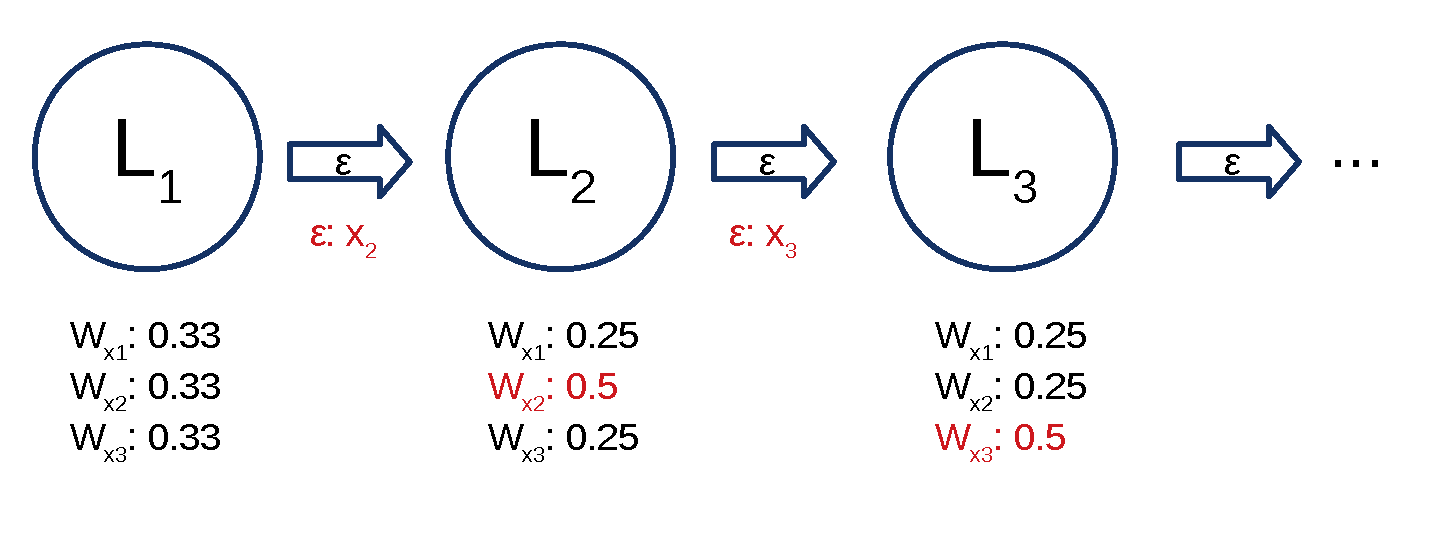
\includegraphics[width=\columnwidth]{boosting-batch}
	\caption{Example of batch boosting. After the ensemble makes an error for an instance, we
	increment the weight for that instance, and train the new learner using the updated
	weights.}
	\label{fig:boosting-batch}
\end{figure}


Online boosting has found more widespread use compared to online bagging ensembles,
as it has been used successfully in many computer vision applications, with a focus on
object tracking \cite{online-boost-cv4, online-boost-cv, online-boost-cv3, online-boost-cv2, online-boost-cv5, online-boost-cv-6, online-boost-cv-7}.
As a result many different boosting algorithms have been proposed, some aimed at a specific application like object tracking, and others that are general learning algorithms.

We will focus on the original algorithm proposed by \citeauthor{Oza2001online},
which we also make use of in \boostvht,
and the more recent general online boosting algorithms that improve upon the
theoretical guarantees and performance of the original.

The original online boosting algorithm by \citeauthor{Oza2001online}, referred to as
OzaBoost, is listed
in Algorithm \ref{alg:ozaboost}.
The learning process is similar to that of OzaBag (Algorithm \ref{alg:ozabag}), but now the
algorithm is strictly sequential, and the weight the example takes depends on whether
the previous member of the ensemble was able to correctly classify the example.
Specifically, the algorithm tries to assign half the total weight to the misclassified
examples on the next stage, and the other half to the correctly classified ones.
This is done by keeping track of the $\lambda$ parameter sums for the two cases,
correct and incorrect classification. We update the weight of an example
before it passes on to the next member of the ensemble accordingly, increasing
the weight every time is incorrectly classified, and decreasing it every time it
is correctly classified.  One thing to note about OzaBoost is that it requires
that we set the number of boosting rounds from the beginning, unlike the
batch AdaBoost algorithm. A simplified illustration of the algorithm is given
in Figure \ref{fig:boosting-online}


\begin{figure}
	\centering
	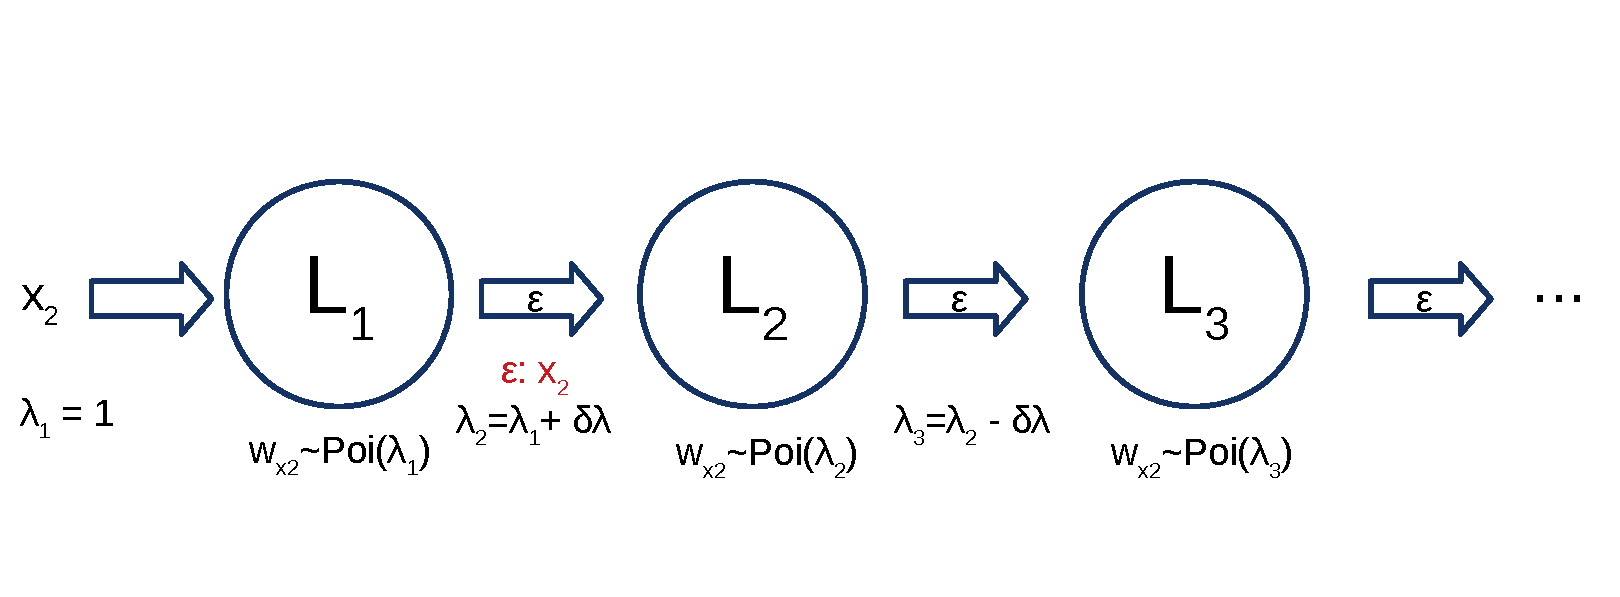
\includegraphics[width=\columnwidth]{boosting-online}
	\caption{Example of online OzaBoost. The instance $x_2$ passes through each learner in sequence.
	Its weight is drawn from a Poisson distribution, whose $\lambda$ parameter is increased
	when a learner makes an error, and decreased otherwise. Here $L_1$ makes an error, while
	$L_2$ correctly classifies the instance.}
	\label{fig:boosting-online}
\end{figure}

Despite its popularity, OzaBoost lacks rigorous theoretical guarantees.
The first attempt to formalize online boosting was made by \citet{online-boosting-theoretical}.
They re-visit the assumption made about the performance of the weak
learners, namely that any weak learner will be able to
do better than random guessing, as it is not a realistic assumption
for the online setting where learner accuracy is more limited. They also
provide a way to not have to set the number of learners in the ensemble beforehand,
by dynamically assigning voting weights to learners.
However, doing so requires the setting of another parameter $\gamma$,
for which it is hard to determine good values.
Their algorithm, OSBoost,
extends the batch SmoothBoost \cite{smoothboost} algorithm, which
was designed as a boosting algorithm robust to noise, to the online
setting. They use the weighting scheme from that algorithm to assign
larger weights to incorrectly predicted examples, and prove that
their ensemble can use the set of weak learners to achieve a small
error.

The work of \citet{Beygelzimer2015optimal} improves upon OSBoost,
by providing an optimal algorithm in terms of ``the number of weak learners
and the sample complexity needed to achieve a specified accuracy'', and also provides
a parameter-free algorithm that does away with the need to set the $\gamma$
parameter of OSBoost.
The optimal algorithm, Online.BBM, is based on the Boost-by-majority batch
algorithm \cite{batch-bbm} and relaxes the assumptions made by OSBoost,
while the parameter-free algorithm, AdaBoost.OL, makes use of online
loss minimization where \citeauthor{Beygelzimer2015optimal} choose to minimize logistic loss
in order to avoid large weights which could adversely affect the
error rate of the algorithm.
We should note that all the above algorithms are strictly sequential
and are therefore hard to parallelize.
Our work in \boostvht is able to
make use of any online boosting algorithm to perform
parallel online boosting, while maintaining their guarantees.


\begin{algorithm}
	\small
	\caption{OzaBoost(\ensemble, $L_o$, $(x,y)$)}
	\label{alg:ozaboost}
	\Initialization{$\lambda^c_t \define \lambda^w_t \define 0 , \quad \forall t \in [1,s]$
		\tcp*[f]{cumulative weight of instances with correct and wrong predictions}}
	\Input{\ensemble, the ensemble, a set of $s$ hypotheses $h_t$;
		$L_o$, an online learning algorithm;
		$(x,y)$, a labeled training instance.}
	\Output{prediction $\widehat{y}$.}
	\tcp*[h]{prequential evaluation: first test...} \;
	$\widehat{y} = \argmax_{\dot{y} \in Y} \sum_{t = 1}^{s} \log \left( \frac{1-\epsilon_t}{\epsilon_t} \right) I\left( h_t(x) = \dot{y} \right)$ \;
	\tcp*[h]{...then train} \;
	$\lambda \define 1$\;

	\ForEach(\tcp*[f]{in order $t \in [1,s]$}){$h_t \in \ensemble$}{
		k \define Poisson($\lambda$) \;
		\While(\tcp*[f]{give weight $k$ to the instance}){k > 0}{
			$h_t \define L_o(h_t, (x,y))$ \;
			$k \define k-1$ \;
		}
		\If(\tcp*[f]{correct prediction}){$y = h_t(x)$}{
			$\lambda^c_t \define \lambda^c_t + \lambda$ \;
			$\epsilon_t \define \frac{\lambda^w_t}{\lambda^c_t + \lambda^w_t}$ \;
			$\lambda \define \lambda \left( \frac{1}{2(1 - \epsilon_t)} \right)$ \;
		}\Else(\tcp*[f]{wrong prediction}){
			$\lambda^w_t \define \lambda^w_t + \lambda$ \;
			$\epsilon_t \define \frac{\lambda^w_t}{\lambda^c_t + \lambda^w_t}$ \;
			$\lambda \define \lambda \left( \frac{1}{2 \epsilon_t} \right)$ \;
		}
	}
	\Return $\widehat{y}$ \;
\end{algorithm}



%\section{Drift Adaptation}
%\label{sec:bg-ol-adapation}

\section{Evaluation}
\label{sec:bg-ol-evaluation}

The evaluation of online learning algorithms differs from the batch
case, not only because of the potential for a concept drift occurring,
but also due to considerations about the computational cost of the
methods themselves. The research on valid evaluation methods for
streaming methods is somewhat limited however, with the notable exception
of the work by \citet{online-evaluation-kdd}, further expanded in
\cite{online-evaluation-journal}\todo{Maybe mention "The comparison and Evaluation of Forecasters"}.
In this section we provide
a brief overview of the challenges and proposed solutions for
the evaluation of online learning algorithms and refer the
reader to \cite{online-evaluation-journal} for an in-depth look
into these issues.

\citet{online-evaluation-journal} identify three areas that
become important in the evaluation of streaming learning
algorithms: \emph{Space} in terms of the memory requirement of the algorithm, \emph{learning time}, and \emph{generalization power}.
Each of these aspects is important in the online learning scenario, and
we will discuss here the space and generalization power aspects, since
learning time is a more intuitive concept.


Online learning algorithms are commonly designed for limited resource environments,
and as such, the space requirements of the algorithm are an important consideration.
Apart from the theoretical analysis of the space cost of the algorithms,
their empirical costs should also be analyzed, as the empirical differences
between algorithms with the same theoretical memory cost can be
significant. \citet{ram-hours} introduced
the concept of \emph{RAM-hours} for this purpose, with the aim of estimating
the cost-efficiency of an algorithm in a cloud environment where instances
are charged according to the time taken to use them, and instances with
higher memory capacities are usually more expensive.
RAM-hours measure the empirical memory consumption of an
algorithm, with one GB of RAM deployed for an hour equaling one RAM-hour.
\citet{vfdt}
make specific mention of the memory requirements of the online decision
tree algorithm they develop, and provide solutions that make the algorithm
memory bounded. However as \citet{online-evaluation-journal} mention, this
is an aspect often overlooked in the evaluation of online learning
algorithms.

In terms of evaluating the generalization power of online learning
algorithms, one aspect that requires special attention is the fact
that the learner evolves as we train it with more samples, so its
performance in the early stages of learning can be very different
to later stages. The two strategies proposed as viable evaluation strategies for the online
setting in \cite{online-evaluation-journal} are \emph{holdout testing}
and \emph{prequential evaluation}. Holdout testing refers to the
established evaluation method from batch learning, where we train
our algorithm on a subset of the data, the \emph{training set},
and evaluate its performance on a set of unseen data, the
\emph{test set} or \emph{holdout set}. This requires us to set a
specific interval at which we check the performance of the algorithm
on the test set, although theoretically we could also perform this
test after each example, introducing however a large computational overhead if
the test set is large.

An alternative is to use
predictive sequential (prequential) evaluation where we present
an example to the algorithm, make a prediction, update our metric,
and finally reveal the example's label and proceed to train the
algorithm with it. This method can also be used in situations
where the label is available for only few of the points in the
data set. However, because the model will exhibit worse performance
in the early learning stages, it is recommended to apply a forgetting
factor to the metric, so that large errors made in the start do
not severely affect the overall evaluation of the algorithm. This
can be done using sliding windows, i.e. evaluating the error using
overlapping subsets of the incoming dataset, or using fading
factors which discount the error for older examples \cite{online-evaluation-kdd}.
These have the added advantage of being faster to compute and memory-less
compared to using sliding windows.

One common issue in classification, in the batch as well as the online setting, is class
imbalance.
For example, on a dataset where 90\% of the instances belong to a single
class, a simple majority classifier will achieve 90\% accuracy, although no
real learning is taking place.
To deal with this problem in the online setting, \citet{kappa-statistic}
proposed the Kappa statistic, and its extension $\kappa_m$ \cite{kappa-m},which is a robust estimator that takes into consideration
the probability that a classifier will produce the correct prediction by chance.
The metric has also been expanded to deal with temporal dependence
in the labels of subsequent examples \cite{temporal-dependence}.
More recently, \citet{prequential-auc} proposed an online adaptation
of the area under the ROC curve metric (AUC) \cite{auc}, called
\emph{prequential AUC} which can deal with the class-imbalance
problem also in the presence of concept drift, and performed
an evaluation against metrics like the Kappa statistic to show
that each metric captures a different aspect of the algorithm's performance.

\section{Software}
\label{sec:bg-ol-software}

Compared to the multitude of options available for batch learning, the availability
of open-source software for online learning is relatively limited. In this section we
mention the most popular libraries for online learning, and point out the ones we have have used
and extended as part of this dissertation.

Perhaps the first online learning library released was the Very Fast Machine Learning (VFML) framework which was developed by \citet{vfdt} as part of their work on the Very Fast Decision Tree (VFDT) algorithm (which we describe in Chapter \ref{sec:bg-dt-online-trees}).
It includes the VFDT and its variations, as well as data pre-processing tools.

One of the most established open-source frameworks for online learning is MOA, which stands
for Massive Online Analysis \cite{bifet2010moa}. MOA includes a collection of
learning algorithms, evaluation methods and metrics, data generators as well as
a graphical interface to perform repeatable experiments. MOA is designed in the
vein of WEKA \cite{weka} and includes interfaces that allow inter-operability
between the algorithms available in WEKA and MOA. Like WEKA, MOA has an extensible
design that allows developers to re-use parts of the existing algorithms to develop
new methods, and easily evaluate new methods using the evaluation strategies mentioned
in Section \ref{sec:bg-ol-evaluation}, by adhering to a simple API. In our work,
we have used MOA to implement the algorithms of \uncertaintrees and as a baseline comparison
in \boostvht. Other single-worker online learning libraries
include LIBOL~\cite{libol} and more recently scikit-multiflow~\cite{sk-multiflow}.

One drawback of these libraries is that they are designed to run on a single machine and therefore
can have issues with massive, distributed streams. Apache SAMOA \cite{samoa} is an effort
to bring the design principles of MOA into the distributed setting, utilizing a platform-independent
design that allows it to run on top of many distributed stream processing engines like
Apache Flink \cite{flink}, Apache Storm~\cite{storm} and Apache Samza~\cite{samza}.
Similarly to MOA, it provides learning algorithms and evaluation methods, and its
design makes it easy to extend with new algorithms.
We have used SAMOA as the development framework for \boostvht.

Another library aimed at distributed stream learning is the StreamDM library~\cite{streamdm}.
StreamDM also inherits some of the design aspects of MOA, providing similar interfaces
to access learning algorithms and run evaluations, but unlike SAMOA
is built to run on top of only the Apache Spark~\cite{spark} streaming engine.
While running on top of a distributed stream engine can make the development
of distributed algorithms easier, it can have a negative effect on the
performance of the library, due to the overhead introduced by the
engine. To tackle this is issue, an optimized version of StreamDM
was proposed in \cite{streamdmPP}. An earlier attempt at developing
a distributed streaming learning framework was Jubatus~\cite{jubatus}.

Finally, one of the most successful frameworks that relies on online learning,
albeit to deal with batch problems, is Vowpal Wabbit (VW) \cite{vw}. VW makes
use of parallel and distributed Stochastic Gradient Descent \cite{sgd} as its main
learning algorithm and has been extended to provide a number of online learning models,
including online boosting \cite{Beygelzimer2015optimal}, online Latent Dirichlet Allocation
\cite{ldaOnline}, and contextual bandits \cite{onlineBandits}.
